

\chapter{Étude de la structure d'un flot de liens}

L'étude de la structure des réseaux est un sujet qui est étudié depuis assez longtemps \REF.
Ces études ont, dans un premier temps, permis de trouver comment caractériser une structure puis, dans un second temps, de proposer des méthodes de détections de ces structures.
La littérature sur l'étude des flots de liens est encore récente et il n'existe que peu d'études \REF sur les spécificités des structures dans les flots de liens.
Nous nous intéressons à une archive de courriels publiquement disponibles\footnote{\url{https://lists.debian.org/debian-user/}}.
Cette archives l'ensemble des courriels échangés par différent utilisateurs lors de l'utilisation de debian.
Typiquement, une personne ayant un problème lors de l'installation envoie un courriel à la liste afin de demander de l'aide.
Toutes personnes inscrites sur la liste reçoit cette demande et peut y répondre.
Ces données se transposent facilement sous forme de flot de liens car une personne est un n\oe uds et chaque courriel entre deux personnes donne lieu à un lien dans le flot à l'instant où le courriel a été envoyé.
Le message initiant la conversation est ignoré pour éviter les boucles.
L'avantage de ces données de communications est que nous connaissons la discussion dans laquelle a lieu chaque message.
Une discussion est un ensemble de courriels dont tout les messages répondent à un message précédant excepté pour le premier qui a initié la discussion et que nous appelons $racine$.
Ainsi, nous étudions la structure des discussions dans le flot liens représentant les courriels envoyés sur la liste.

Utiliser le formalisme de flot de liens est particulièrement intéressant car cette lite de diffusion existe depuis 1994.
L'aspect temporelle des discussion est donc important.



\section{Prétraitement sur le jeu de données}
Bien que disponible, ce jeu de données nécessite un ensemble de traitement avant de pouvoir exploiter les 724985 courriels que contenait l'archive en janvier 2015.
Tout d'abords, les données ne sont pas sous la forme d'un flot de liens avec la structure des conversations.
Les données sont accessibles via le site internet.
Pour avoir ces informations sous la forme d'un flots de liens, un script d'extraction a été développé \com{URL}.
Lors de l'extraction, 2269 courriels n'ont pas pu être pris en compte car certaines informations étaient manquantes ou mal formées.

Une fois les informations récupérées, il est nécessaire de vérifier leurs cohérences.
Pour chaque courriel, la date et l'heure d'envoie, l'auteur, le destinataire, le courriel auquel il répond et la discussion dans laquelle il apparait sont connus.
Un message peut être filtré pour différentes raisons: le courriel apparait avant le message auquel il est censé répondre, le message auquel il réponds n'est pas présent dans l'archive, l'auteur et le destinataire sont la même personne\footnote{Ce cas est relativement rare.}.
Il s'agit de vérifications simple auquel il faut ajouter les vérification de la cohérence de la structure de discussions.
Ainsi, une discussion est retirée du jeu de donnée si il manque la racine, un de ces messages a été retiré précédemment ou si la discussion a débuté trop récemment ou si elle dure trop longtemps.
Les deux dernières conditions permettent d'éviter un biais envers les conversations incomplètes car trop longues ou trop récentes.

Une fois tout ces messages filtrés, nous obtenons un flot de liens avec 554233 liens entre 34648 personnes pendant presque 19 ans et 116999 discussions.
Mis à part les courriels de début de discussions, ce sont 53753 courriels qui ont été filtrés car incohérents.

\section{Caractéristiques des threads (COMPLENET)}

\begin{figure}[!h]
\centering

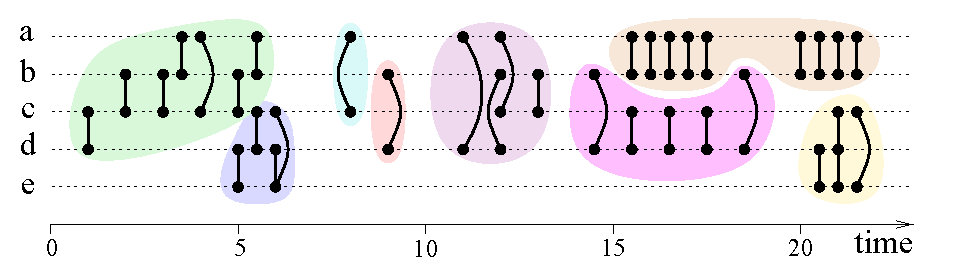
\includegraphics[width=0.9\linewidth]{img/flot_communautes.eps}
\caption{An example of link stream representing email exchanges between individuals $a$, $b$, $c$, $d$ and $e$, with threads represented by colored areas. For instance, at time $5$, $b$ and $c$ exchange an email, as well as $d$ and $e$. Threads are {\em a priori} dense series of exchanges involving a limited group of nodes during a limited period of time.
% The more classical graph modeling of such data is displayed in Figure~\ref{fig:communities-in-g}.
}
\label{fig:threads-in-ls}
\end{figure}